\documentclass[10pt, conference, compsocconf]{IEEEtran}
\usepackage{cite}
\usepackage{subfigure}
\ifCLASSINFOpdf
\usepackage[pdftex]{graphicx}
\graphicspath{{pdf/}{figures/}}
% and their extensions so you won’t have to specify these with
% every instance of \includegraphics
\DeclareGraphicsExtensions{.pdf,.jpeg,.png}
\else
% or other class option (dvipsone, dvipdf, if not using dvips). graphicx
% will default to the driver specified in the system graphics.cfg if no
% driver is specified.
\usepackage[dvips]{graphicx}
% declare the path(s) where your graphic files are
\graphicspath{{…/eps/}}
% and their extensions so you won’t have to specify fthese with
% every instance of \includegraphics
\DeclareGraphicsExtensions{.eps}
\fi

\usepackage{array}
\usepackage{multirow}
\usepackage{longtable}
\usepackage{rotating}
\usepackage[cmex10]{amsmath}
\usepackage{algorithmic}
\usepackage{array}
\usepackage{mdwmath}
\usepackage{mdwtab}
\usepackage{stfloats}
\usepackage{url}
\usepackage[colorlinks,
linkcolor=blue,
anchorcolor=blue,
citecolor=blue]{hyperref}
\hyphenation{op-tical net-works semi-conduc-tor}


\begin{document}
	%
	% paper title
	% can use linebreaks \\ within to get better formatting as desired
	\title{Document Scanner Based on PaddlePaddle}
	
	\author{\IEEEauthorblockN{Chang Lu$^1$\IEEEauthorrefmark{0},
			Xiaochun Lei$^{* 1,2}$\IEEEauthorrefmark{0},
			Junlin Xie$^1$\IEEEauthorrefmark{0}, 
			Xiaolong Wang$^1$\IEEEauthorrefmark{0} and
			XiangBoge Mu$^1$\IEEEauthorrefmark{0}}
		\IEEEauthorblockA{\IEEEauthorrefmark{0}1.School of computer and information security,\\
			Guilin University of Electronic Technology,
			Guilin 541004, China;}
		\IEEEauthorblockA{\IEEEauthorrefmark{0}2.Guangxi Key Laboratory of Image and Graphic Intelligent Processing, \\Guilin 541004, China;}
		\IEEEauthorblockA{\IEEEauthorrefmark{1}Corresponding author's e-mail: glleixiaochun@qq.com}}
	% use for sepcial paper notices
	%\IEEEspecialpapernotice{(Invited Paper)}
	% make the title area
	\maketitle
	\begin{abstract}
		
	Document scanning aims at trasferring the documents in captured photographs into scanned document files. 
	And with the need of convience to gain contents in documents increasing, it is becoming applied to a wide variety of fields nowadays. 
	However, there also came out some problems such as the low accuracy of document positioning, the vagueness of processing results, the bad quality of scanned images, etc. 
	In this paper we proposed a document processing system based on Semantic Segmentation, which has a great MIoU rank 97.255 and a perfect document processing functionality. 
	The system use OCRNet to segment documents out meanwhile we make use of Ohem cross entropy loss function to optimize the scanned results. 
	And after that, we use affine transformation and other post-processing algorithms according to the segmentation results to gain the well-scanned documents.
	\end{abstract}
	
	\begin{IEEEkeywords}
		
		Document Scanner, Document Processing, Semantic Segmentation.
		
	\end{IEEEkeywords}
	
	\IEEEpeerreviewmaketitle
	
	\section{Introduction}
	
	% introduce background

	Document scanning systems have been mature and widely used in amounts of fields such as official business, administration and so on. 
	With the demand of on-device document scanning increasing, systems for document scanning are proposed in order to provide office crowd with convience. 

	% bring out problems

	Originally, for most of the systems like hough transformation!!!, key point regression!!!, the accuracy of document positioning, the legibility of document scanning and the quality of scanned images all cannot satisfy people's needs. 

	% introduce OCRNet

	OCRNet, a object-contextual representation system based on semantic segmentation, is used to be the major component of the system we proposed. 

	% take a statement why use it

	The reasons for choosing it are: 
	
	It solved the context aggregation problem in semantic segmentation by making use of target regional representations to enhance its pixel representations, which evidently improves the quality of segmentation results. 
	The OCR method it mainly uses is light-weighted, effective, rapid and easy to train.  

	% show its MIoU

	And it reached 94.14 MIoU score based on baidu opensource dataset. 

	% introduce post processing section

	After we gain the result from OCRNet, we will have it post processed. 
	First, we recognize background color of raw scanned images in it. 
	Then, we separate foreground color out according to various threshold values of background colors. 
	After that, we choose several representive color from foreground colors as index colors. 
	Last, we change the colors in origin image by index colors. 
	
	\section{Methods}
		\subsection{System Design}

		% show flow charts

		\begin{figure}[!h]
			\centering
			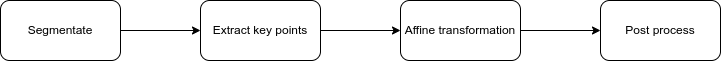
\includegraphics[width=2.3in]{./Assets/FlowChart.png}
			\caption{System Procedure}
		\end{figure}

		% give the statements.

		The procedure of our system is: 
		First, we use OCRNet to segmentate out the documents in pictures. 
		Second, we extract out the key points to position the documents. 
		Third, we affine the key points to become normal. 
		The last, we get the results post processed. 

		\subsection{System Implementation}

			\subsubsection{Image Segmentation}

			% introduce the details of OCRNet

			Yuhui Yuan et al proposed OCRNet, a Object-Contextual Representations network for semantic segmentation. 
			It use the construction made up of HRNet, OCR and SegFix. 
			Thereinto, OCR method is divided to three stages. 
			First, it obtains feature representations from backbone network and then estimates a rough semantic segmentation. 
			The result will be the input of OCR method and named soft object regions.
			Second, it computes $k$ vector groups according to soft object regions and feature representations and then make it as object region representations. 
			Third, it computes the relational matrix of pixel representations from the network's bottommost layer and object region representations. 
			Then it computes the weighted summation of the object region features based on the value of each pixel and the object region feature represented in the relationship matrix. 

			% compare it with U-Net
			By comparing OCRNet with U-Net, we find that U-Net will generate segmentation region cavities while OCRNet won't. 
			We input baidu opensource dataset to these networks and get the results they generated. 
			For those results they generated, it's obvious to find that U-Net generate some holes in some segmentation regions. 
			Meanwhile we learnt that OCRNet generate almost no holes at the same segmentation regions. 
			Therefore we use OCRNet to structure the system. 
			
			% Show the constructure of OCRNet

			\begin{figure}[!h]
				\centering
				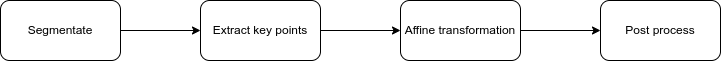
\includegraphics[width=2.3in]{./Assets/FlowChart.png}
				\caption{OCRNet Construction}
			\end{figure}

			% state the loss: OhemCrossEntropyLoss and DiceLoss

			Different from OCRNet, we use Ohem cross entropy loss and dice loss to optimize the network. 

			Ohem cross entropy loss, as known as online hard example mining cross entropy loss, is used to pay close attention to hard examples and set higher weight of them. 
			The definition of Ohem cross entropy loss is:
			$$
			L_{Ohem} = -\log\bigg( \frac{\exp(prediction[groundtruth])}{\sum_i \exp(prediction[i])} \bigg)
			$$
			Thereinto, $prediction$ is a probability density function on groundtruth and $prediction[groundtruth]$ is the probability of prediction on the label of corresponding groundtruth. 

			dice loss, proposed by V-Net!!!, is derived from dice coefficient and often seen as a metrical function to estimate comparability of two samples. 
			The definition of dice loss is: 
			$$
			L_{dice} = 1 - \frac{2|prediction\cap groundtruth|}{|prediction| + |groundtruth|}
			$$
			Thereinto, $|prediction\cap groundtruth|$ is the intersection between prediction and groundtruth, $|prediction|, |groundtruth|$ is the number of aggregate prediction and groundtruth. 
			We set the weight of Ohem cross entropy loss to 1 and the weight of dice loss to 0.2, then combine them into a mixed loss function.  

			\subsubsection{Document Processing}

			% fitting the keyt points
			% https://blog.csdn.net/ooooocj/article/details/110936343
			We use Douglas-Peucker algorithm to fit the key points. 
			We first sample from the curve, extract finite points and connect them with lines. 
			Meanwhile, we use these lines to keep the original shape of the curve. 
			
			

			% affine trasfromation
			After we finish fitting key points, we use getPerspectiveTransform and warpPerspective to affine the key points in order to reshape the scanning results to the normal shape.
			% Affine Or Perspective ?
			% https://cloud.tencent.com/developer/article/1638969
			% https://blog.csdn.net/Caesar6666/article/details/104158047
			First we set up coordinate axis system of the fitted result, get base points of the fitted result, and then set the target points of the normal view. 
			Then we compute the transformation matrix according to the two groups of points. 
			Last we use the matrix to operate the fitted result and then we will get the normal view. 
			It is equivalent to that we have it transformed into the normal view by translating, rotating, scaling, shearing.

			\subsubsection{Post Processing}

			% why use it : make image clear & keep colorful (maybe need to mention the low space usage).
			When we get the result from Document Processing, we still need to post process it. 
			We aim at making images clear and keeping documents colorful. 
			Furthermore, it can minimize the images, which is easy and effective to do other oprations like image fixing, image superresolution, etc.

			% recognize background color of raw scanned images
			First we obtain background colors from the raw scanned images.
			
			% separate foreground color out according to various threshold values of background colors
			Then we separate foreground colors out according to various threshold values of background colors by transfer RGB format into HSV format. 
			The reason we choose HSV is that it can easily recognize the lightness and the saturation value of each color. 
			It enable us to filter those unrepresentative color by setting the thresholds of the difference between lightness and hue value or between saturation and hue value. 

			% choose several representive color from foreground colors as index colors
			The next we select representive colors as index colors from the rest. 
			And last, we change the less representive colors with corresponding index colors. 

	\section{Experiments}

	% the experiment software & hardware environment

	% the used dataset
	We use Baidu opensource dataset to go experiments. 

	% the algorithm comparition between OCRNet and UNet. Attached some pictures.
	We run prediction functionalities of OCRNet and U-Net and then obtaind some results. 

	\begin{figure}[!h]
		\centering
		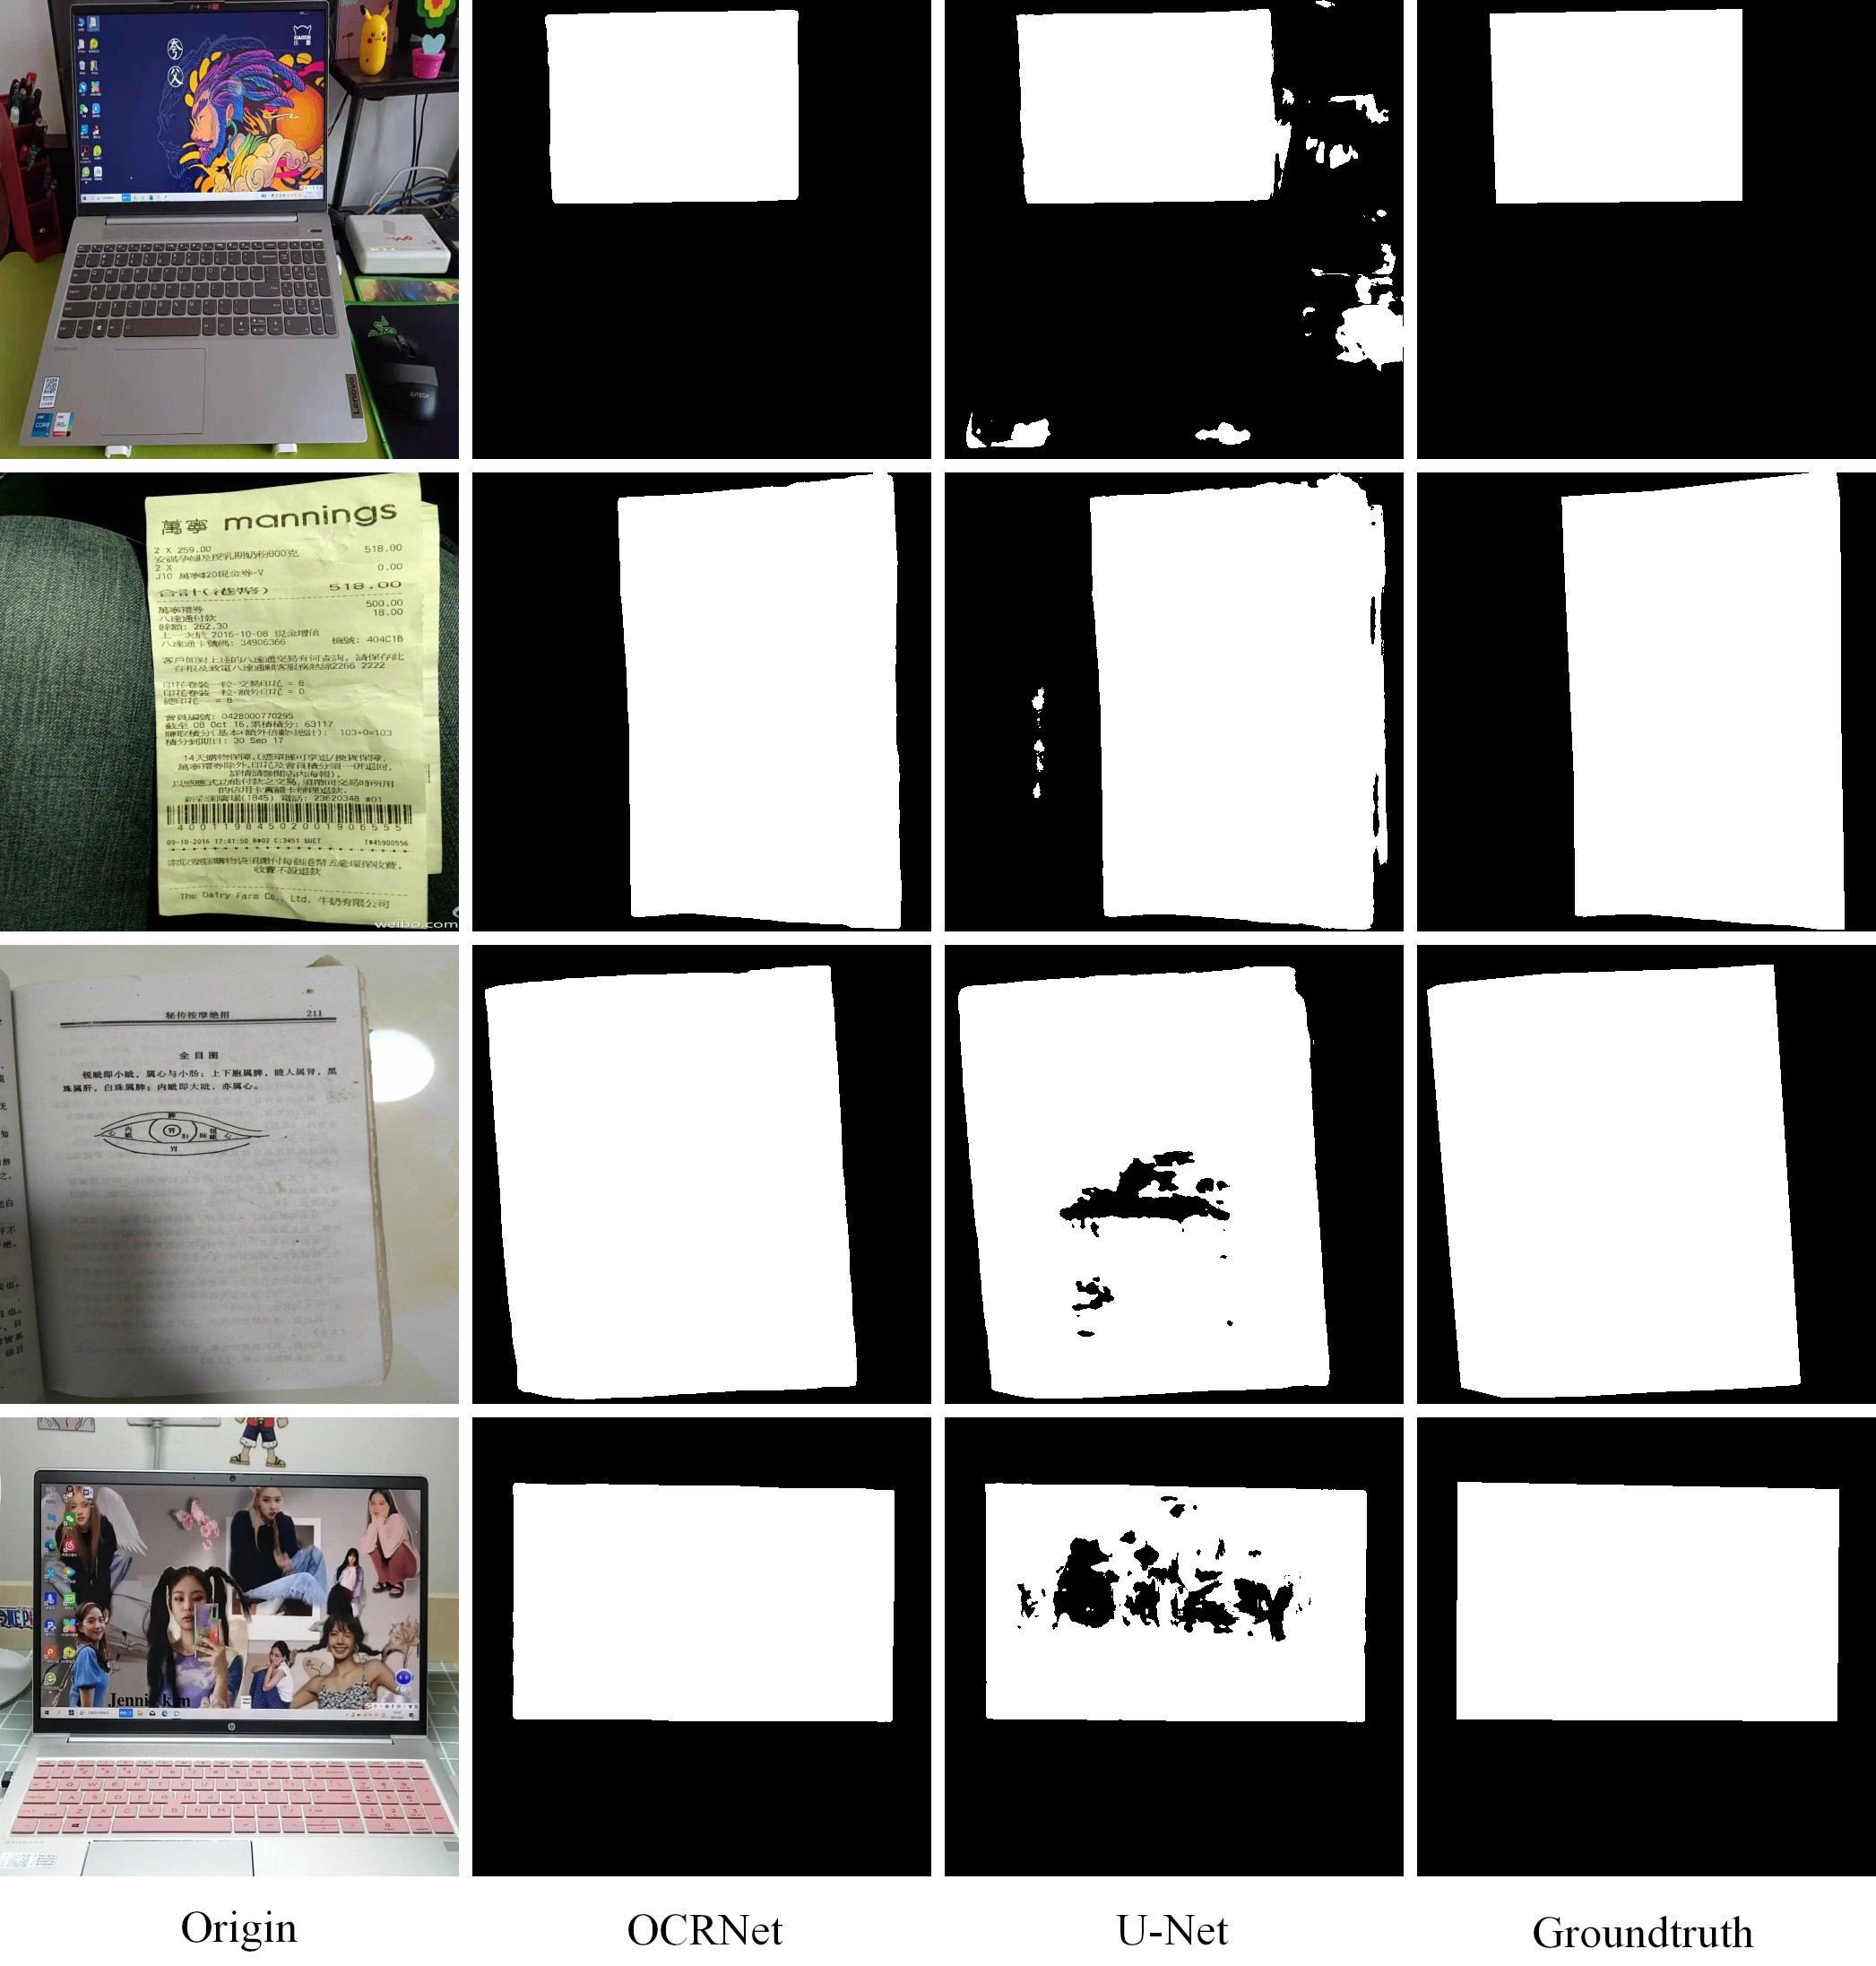
\includegraphics[width=2.3in]{./Assets/final_whole_img.jpg}
		\caption{Comparition between OCRNet and UNet}
	\end{figure}

	It's obvious that some masks generated by U-Net have some holes while those makss generated by OCRNet have no holes. 
	The reason is that OCRNet explicitly enhances the contribution of pixels from the same class of objects when constructing contextual information. 
	And it solved the problem that UNet is not good at modeling continuous large regions. 

	% the post processing containing adaptive Binarization thresold. 
	We use adaptive Binarization threshold process to obtain the mask of image.
	And we gain background colors, extract foreground colors by transferring into HSV format, then filter out representive colors as index colors and at last change colors with corresponding index colors. 
		
	\begin{table}[!h]
		\renewcommand{\arraystretch}{1.3}
		\caption{The Comparison Of Models' MIoU on baidu opensource dataset}
		\centering
		\begin{tabular}{cc} \\
			\hline
			Model & MIoU\\
			\hline
			OCRNet(Origin) & 94.14\\
			\hline
			U-Net & 94.46\\
			\hline
			OCRNet(Ours) & 97.255\\
			\hline
		\end{tabular}
		
	\end{table}
	
	\section{Summmary And Conclusion}

	We build up a document scanning system, which can generate clear and colorful results in good quality. 
	The system is based on OCRNet and it is extended post process to improve the result of OCRNet. 
	And we use baidu opensource dataset to improve the quality of model training. 
	Lastly we make up a mixed loss function combining Ohem cross entropy loss and dice loss to train the model in order to enhance the ability of model processing. 
	
	% use section* for acknowledgement
	\section*{Acknowledgment}
	
	%This essay is supported by Project to Improve the scientific research basic ability of Middle-aged and Young Teachers (No.2019ky0222,2020KY05033),the Open Funds Guangxi Key Laboratory of Image and Graphic Intelligent Processing, No.GIIP2004, Student's Platform for Innovation and Entrepreneurship Training Program under Grant (No.202010595053. 202010595022)
	
	% trigger a \newpage just before the given reference
	% number - used to balance the columns on the last page
	% adjust value as needed - may need to be readjusted if
	% the document is modified later
	%\IEEEtriggeratref{8}
	% The "triggered" command can be changed if desired:
	%\IEEEtriggercmd{\enlargethispage{-5in}}
	
	% references section
	
	% can use a bibliography generated by BibTeX as a .bbl file
	% BibTeX documentation can be easily obtained at:
	% http://www.ctan.org/tex-archive/biblio/bibtex/contrib/doc/
	% The IEEEtran BibTeX style support page is at:
	% http://www.michaelshell.org/tex/ieeetran/bibtex/
	%\bibliographystyle{IEEEtran}
	% argument is your BibTeX string definitions and bibliography database(s)
	%\bibliography{IEEEabrv,../bib/paper}
	%
	% <OR> manually copy in the resultant .bbl file
	% set second argument of \begin to the number of references
	% (used to reserve space for the reference number labels box)
	
	\begin{thebibliography}{1}
		
		\bibitem{gps}
		W. Da-chuan, "Algorithm of road information acquirement based on GPS and electronic map," 2010 3rd International Congress on Image and Signal Processing, Yantai, 2010, pp. 4174-4178, doi: 10.1109/CISP.2010.5646704.
		% Vyacheslavovich T D, Mikhailovich E A, Petrovich N D. Advanced Hough-based method for on-device document localization[J]. Компьютерная оптика, 2021, 45(5): 702-712.
		% Advanced Hough-based method for on-device document localization

		% Segmentation Transformer: Object-Contextual Representations for Semantic Segmentation

		% Advanced Hough-based method for on-device document localization

		% Real-Time Document Localization in Natural Images by Recursive Application of a CNN
		
	\end{thebibliography}
\end{document}
